% Options for packages loaded elsewhere
\PassOptionsToPackage{unicode}{hyperref}
\PassOptionsToPackage{hyphens}{url}
\documentclass[
]{article}
\usepackage{xcolor}
\usepackage[margin=1in]{geometry}
\usepackage{amsmath,amssymb}
\setcounter{secnumdepth}{-\maxdimen} % remove section numbering
\usepackage{iftex}
\ifPDFTeX
  \usepackage[T1]{fontenc}
  \usepackage[utf8]{inputenc}
  \usepackage{textcomp} % provide euro and other symbols
\else % if luatex or xetex
  \usepackage{unicode-math} % this also loads fontspec
  \defaultfontfeatures{Scale=MatchLowercase}
  \defaultfontfeatures[\rmfamily]{Ligatures=TeX,Scale=1}
\fi
\usepackage{lmodern}
\ifPDFTeX\else
  % xetex/luatex font selection
\fi
% Use upquote if available, for straight quotes in verbatim environments
\IfFileExists{upquote.sty}{\usepackage{upquote}}{}
\IfFileExists{microtype.sty}{% use microtype if available
  \usepackage[]{microtype}
  \UseMicrotypeSet[protrusion]{basicmath} % disable protrusion for tt fonts
}{}
\makeatletter
\@ifundefined{KOMAClassName}{% if non-KOMA class
  \IfFileExists{parskip.sty}{%
    \usepackage{parskip}
  }{% else
    \setlength{\parindent}{0pt}
    \setlength{\parskip}{6pt plus 2pt minus 1pt}}
}{% if KOMA class
  \KOMAoptions{parskip=half}}
\makeatother
\usepackage{color}
\usepackage{fancyvrb}
\newcommand{\VerbBar}{|}
\newcommand{\VERB}{\Verb[commandchars=\\\{\}]}
\DefineVerbatimEnvironment{Highlighting}{Verbatim}{commandchars=\\\{\}}
% Add ',fontsize=\small' for more characters per line
\usepackage{framed}
\definecolor{shadecolor}{RGB}{248,248,248}
\newenvironment{Shaded}{\begin{snugshade}}{\end{snugshade}}
\newcommand{\AlertTok}[1]{\textcolor[rgb]{0.94,0.16,0.16}{#1}}
\newcommand{\AnnotationTok}[1]{\textcolor[rgb]{0.56,0.35,0.01}{\textbf{\textit{#1}}}}
\newcommand{\AttributeTok}[1]{\textcolor[rgb]{0.13,0.29,0.53}{#1}}
\newcommand{\BaseNTok}[1]{\textcolor[rgb]{0.00,0.00,0.81}{#1}}
\newcommand{\BuiltInTok}[1]{#1}
\newcommand{\CharTok}[1]{\textcolor[rgb]{0.31,0.60,0.02}{#1}}
\newcommand{\CommentTok}[1]{\textcolor[rgb]{0.56,0.35,0.01}{\textit{#1}}}
\newcommand{\CommentVarTok}[1]{\textcolor[rgb]{0.56,0.35,0.01}{\textbf{\textit{#1}}}}
\newcommand{\ConstantTok}[1]{\textcolor[rgb]{0.56,0.35,0.01}{#1}}
\newcommand{\ControlFlowTok}[1]{\textcolor[rgb]{0.13,0.29,0.53}{\textbf{#1}}}
\newcommand{\DataTypeTok}[1]{\textcolor[rgb]{0.13,0.29,0.53}{#1}}
\newcommand{\DecValTok}[1]{\textcolor[rgb]{0.00,0.00,0.81}{#1}}
\newcommand{\DocumentationTok}[1]{\textcolor[rgb]{0.56,0.35,0.01}{\textbf{\textit{#1}}}}
\newcommand{\ErrorTok}[1]{\textcolor[rgb]{0.64,0.00,0.00}{\textbf{#1}}}
\newcommand{\ExtensionTok}[1]{#1}
\newcommand{\FloatTok}[1]{\textcolor[rgb]{0.00,0.00,0.81}{#1}}
\newcommand{\FunctionTok}[1]{\textcolor[rgb]{0.13,0.29,0.53}{\textbf{#1}}}
\newcommand{\ImportTok}[1]{#1}
\newcommand{\InformationTok}[1]{\textcolor[rgb]{0.56,0.35,0.01}{\textbf{\textit{#1}}}}
\newcommand{\KeywordTok}[1]{\textcolor[rgb]{0.13,0.29,0.53}{\textbf{#1}}}
\newcommand{\NormalTok}[1]{#1}
\newcommand{\OperatorTok}[1]{\textcolor[rgb]{0.81,0.36,0.00}{\textbf{#1}}}
\newcommand{\OtherTok}[1]{\textcolor[rgb]{0.56,0.35,0.01}{#1}}
\newcommand{\PreprocessorTok}[1]{\textcolor[rgb]{0.56,0.35,0.01}{\textit{#1}}}
\newcommand{\RegionMarkerTok}[1]{#1}
\newcommand{\SpecialCharTok}[1]{\textcolor[rgb]{0.81,0.36,0.00}{\textbf{#1}}}
\newcommand{\SpecialStringTok}[1]{\textcolor[rgb]{0.31,0.60,0.02}{#1}}
\newcommand{\StringTok}[1]{\textcolor[rgb]{0.31,0.60,0.02}{#1}}
\newcommand{\VariableTok}[1]{\textcolor[rgb]{0.00,0.00,0.00}{#1}}
\newcommand{\VerbatimStringTok}[1]{\textcolor[rgb]{0.31,0.60,0.02}{#1}}
\newcommand{\WarningTok}[1]{\textcolor[rgb]{0.56,0.35,0.01}{\textbf{\textit{#1}}}}
\usepackage{graphicx}
\makeatletter
\newsavebox\pandoc@box
\newcommand*\pandocbounded[1]{% scales image to fit in text height/width
  \sbox\pandoc@box{#1}%
  \Gscale@div\@tempa{\textheight}{\dimexpr\ht\pandoc@box+\dp\pandoc@box\relax}%
  \Gscale@div\@tempb{\linewidth}{\wd\pandoc@box}%
  \ifdim\@tempb\p@<\@tempa\p@\let\@tempa\@tempb\fi% select the smaller of both
  \ifdim\@tempa\p@<\p@\scalebox{\@tempa}{\usebox\pandoc@box}%
  \else\usebox{\pandoc@box}%
  \fi%
}
% Set default figure placement to htbp
\def\fps@figure{htbp}
\makeatother
\setlength{\emergencystretch}{3em} % prevent overfull lines
\providecommand{\tightlist}{%
  \setlength{\itemsep}{0pt}\setlength{\parskip}{0pt}}
\usepackage{bookmark}
\IfFileExists{xurl.sty}{\usepackage{xurl}}{} % add URL line breaks if available
\urlstyle{same}
\hypersetup{
  pdftitle={Report\_VoserWeber},
  hidelinks,
  pdfcreator={LaTeX via pandoc}}

\title{Report\_VoserWeber}
\author{}
\date{\vspace{-2.5em}}

\begin{document}
\maketitle

\subsection{8.1.1 Physical geography and
phenology}\label{physical-geography-and-phenology}

\begin{enumerate}
\def\labelenumi{\arabic{enumi}.}
\tightlist
\item
  What does the intercept indicate?
\end{enumerate}

The intercept indicates the value of the outcome (DOY) when the
predictor (altitude) is zero.

\begin{enumerate}
\def\labelenumi{\arabic{enumi}.}
\setcounter{enumi}{1}
\tightlist
\item
  How can you interpret the slope?
\end{enumerate}

\begin{Shaded}
\begin{Highlighting}[]
\NormalTok{knitr}\SpecialCharTok{::}\FunctionTok{include\_graphics}\NormalTok{(}\StringTok{"graphs/scatter\_altitude\_doy.png"}\NormalTok{)}
\end{Highlighting}
\end{Shaded}

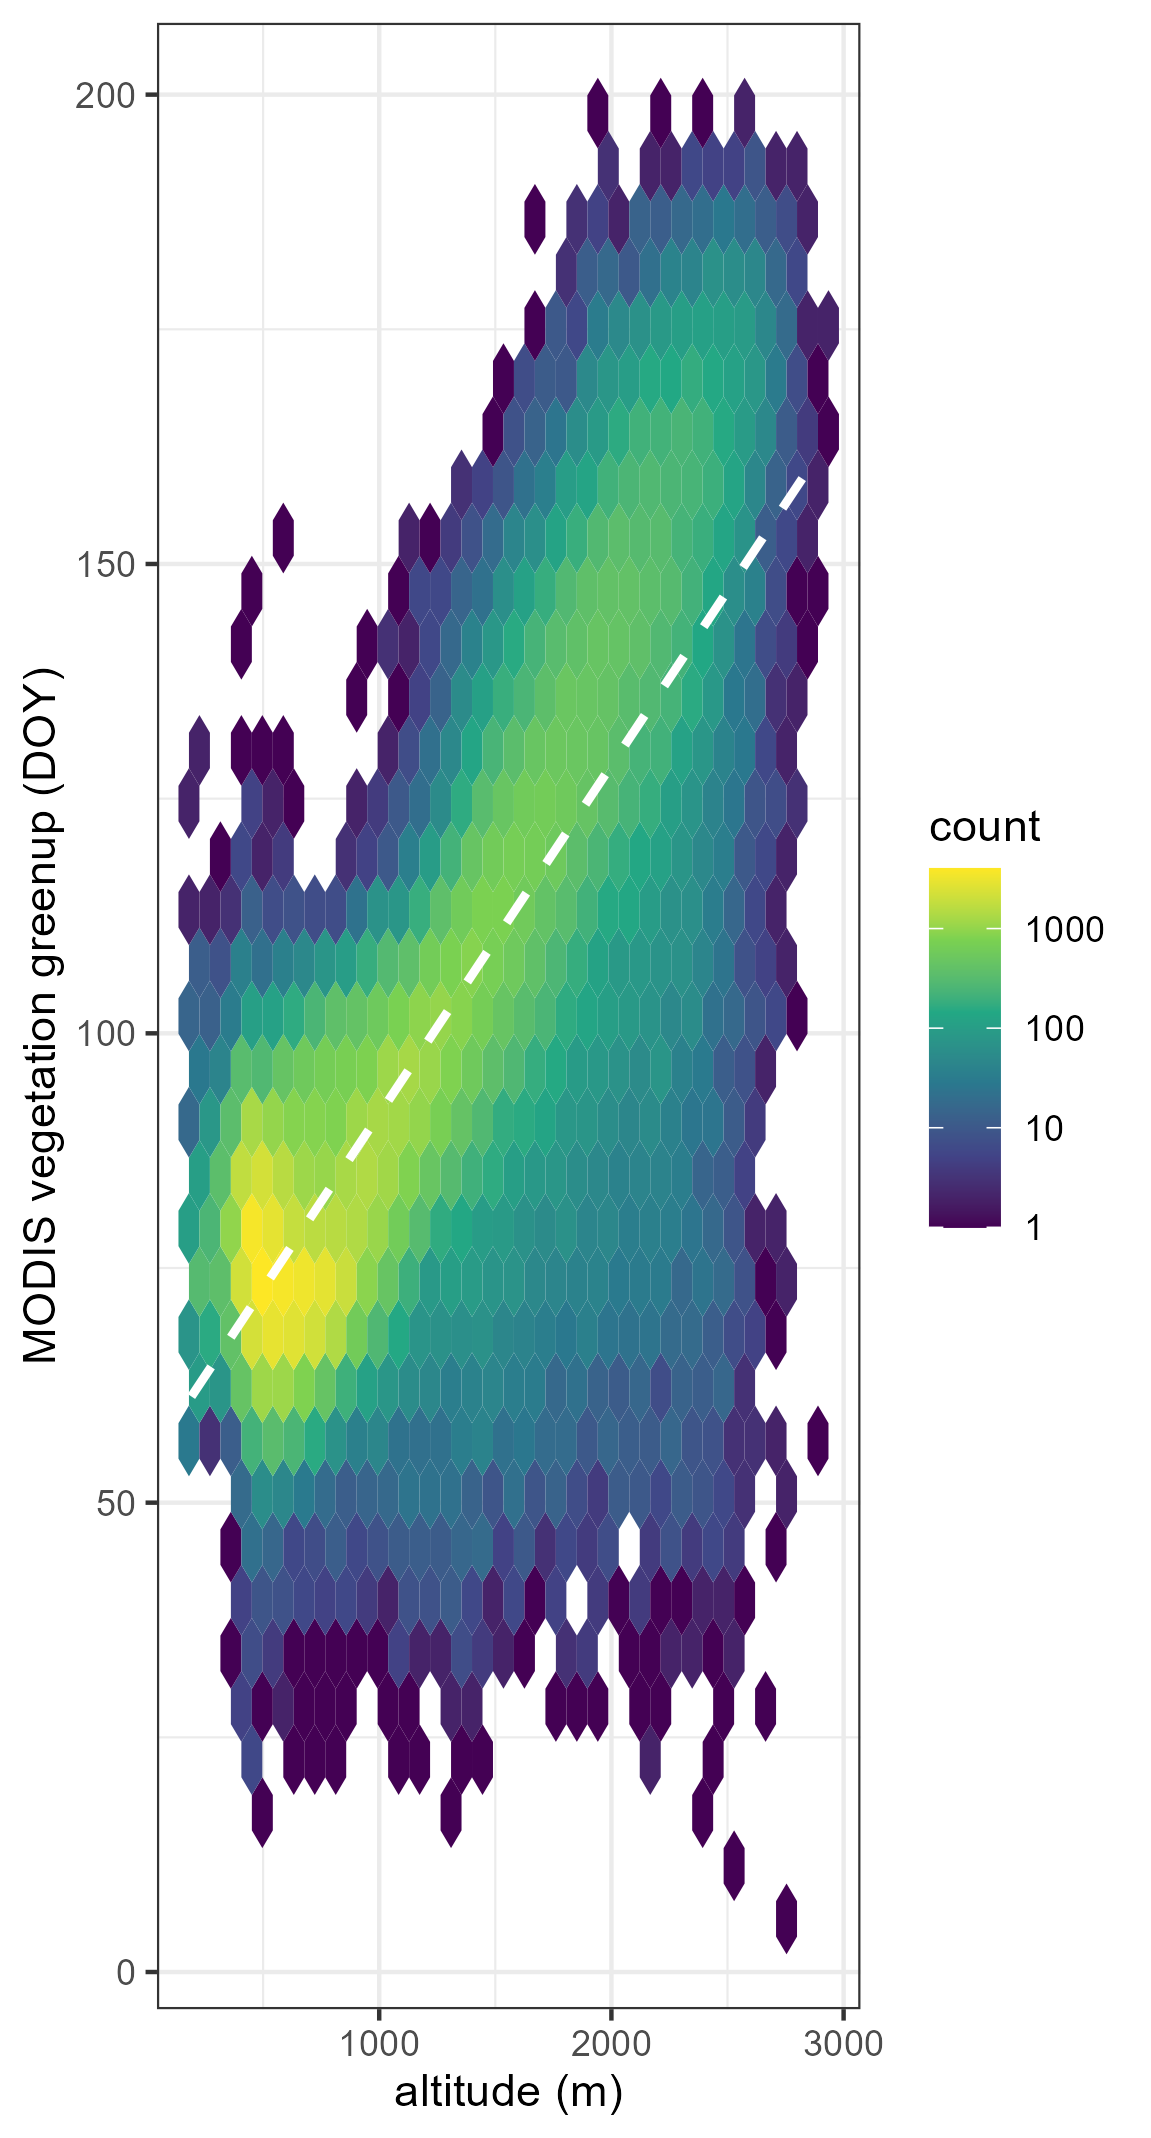
\includegraphics[width=15.99in]{graphs/scatter_altitude_doy}

With higher altitude, the DOY increases (\textasciitilde37 days per
1'000 m of elevation gain), meaning the vegetation greenup is later in
the year.

\begin{enumerate}
\def\labelenumi{\arabic{enumi}.}
\setcounter{enumi}{2}
\tightlist
\item
  How to convert the established relationship with altitude, to one with
  temperature (Without actually doing it, just describe how you would go
  about this and what you would expect? Can you approximate the effect
  of 1 degree of warming?)
\end{enumerate}

Depending on the atmosphere's local water content, air temperature
decreases by 0.5 - 1.0 °C per 100 meters of elevation. This relationship
could be used to create a model which would predict the change of time
in the local vegetation greenup - say the temperature rises by 1 °C (and
the atmosphere is dry), then the vegetation greenup would occur
\textasciitilde3.7 days earlier.

\section{8.1.2 Temporal and spatial
anomalies}\label{temporal-and-spatial-anomalies}

For a location near the Adirondacks in the North-Eastern United States
(Figure 8.1) gather phenology data on both the day of greenup and the
day of maximum canopy development of a location centered on 43.5 N and
74.5 W. Use a product that directly provides these quantities. Gather
data for all pixels 100 km around this location for years 2001 to 2010.
Ensure you have the right region, e.g.~by plotting it
terra::plot(your\_raster). Similarly, download land cover data for the
year 2010 for the same spatial extent, and only consider IGBP broadleaf
and mixed forest classes in your analysis.

For the years 2001 - 2009 calculate the long term mean (LTM) and
standard deviation (SD) of the phenology metrics. Calculate location
with an early greenup for 2010 (\textless{} LTM - 1 SD) and locations
with late maturity (\textgreater{} LTM + 1 SD).

Describe the observed patterns and speculate about the underlying
reasons. In addition, download a digital elevation map for the United
States (30s resolution), and compare differences in altitude (e.g.~a
boxplot) across locations where you do or do not see any patterns in
phenology.

\subsection{Code}\label{code}

\#\#Setup

\begin{Shaded}
\begin{Highlighting}[]
\FunctionTok{library}\NormalTok{(MODISTools)}
\end{Highlighting}
\end{Shaded}

\begin{verbatim}
## Warning: Paket 'MODISTools' wurde unter R Version 4.5.3 erstellt
\end{verbatim}

\begin{Shaded}
\begin{Highlighting}[]
\FunctionTok{library}\NormalTok{(terra)}
\end{Highlighting}
\end{Shaded}

\begin{verbatim}
## Warning: Paket 'terra' wurde unter R Version 4.5.3 erstellt
\end{verbatim}

\begin{verbatim}
## terra 1.9.11
\end{verbatim}

\begin{Shaded}
\begin{Highlighting}[]
\FunctionTok{library}\NormalTok{(tidyverse)}
\end{Highlighting}
\end{Shaded}

\begin{verbatim}
## Warning: Paket 'tidyverse' wurde unter R Version 4.5.3 erstellt
\end{verbatim}

\begin{verbatim}
## Warning: Paket 'ggplot2' wurde unter R Version 4.5.3 erstellt
\end{verbatim}

\begin{verbatim}
## Warning: Paket 'purrr' wurde unter R Version 4.5.2 erstellt
\end{verbatim}

\begin{verbatim}
## Warning: Paket 'dplyr' wurde unter R Version 4.5.3 erstellt
\end{verbatim}

\begin{verbatim}
## -- Attaching core tidyverse packages ------------------------ tidyverse 2.0.0 --
## v dplyr     1.2.0     v readr     2.1.5
## v forcats   1.0.0     v stringr   1.5.2
## v ggplot2   4.0.2     v tibble    3.3.0
## v lubridate 1.9.4     v tidyr     1.3.1
## v purrr     1.2.0
\end{verbatim}

\begin{verbatim}
## -- Conflicts ------------------------------------------ tidyverse_conflicts() --
## x tidyr::extract() masks terra::extract()
## x dplyr::filter()  masks stats::filter()
## x dplyr::lag()     masks stats::lag()
## i Use the conflicted package (<http://conflicted.r-lib.org/>) to force all conflicts to become errors
\end{verbatim}

\begin{Shaded}
\begin{Highlighting}[]
\FunctionTok{library}\NormalTok{(geodata)}
\end{Highlighting}
\end{Shaded}

\begin{verbatim}
## Warning: Paket 'geodata' wurde unter R Version 4.5.3 erstellt
\end{verbatim}

\begin{Shaded}
\begin{Highlighting}[]
\FunctionTok{library}\NormalTok{(tmap)}
\end{Highlighting}
\end{Shaded}

\begin{verbatim}
## Warning: Paket 'tmap' wurde unter R Version 4.5.3 erstellt
\end{verbatim}

\begin{Shaded}
\begin{Highlighting}[]
\CommentTok{\# {-}{-}{-} Parameter {-}{-}{-}}
\NormalTok{lat }\OtherTok{\textless{}{-}} \FloatTok{43.5}
\NormalTok{lon }\OtherTok{\textless{}{-}} \SpecialCharTok{{-}}\FloatTok{74.5}
\NormalTok{years }\OtherTok{\textless{}{-}} \DecValTok{2001}\SpecialCharTok{:}\DecValTok{2010}
\end{Highlighting}
\end{Shaded}

\#\#Daten einlesen

\begin{Shaded}
\begin{Highlighting}[]
\NormalTok{phenology }\OtherTok{\textless{}{-}} \FunctionTok{read.csv}\NormalTok{(}\StringTok{"data{-}raw/phenology.csv"}\NormalTok{)}
\NormalTok{land\_cover }\OtherTok{\textless{}{-}} \FunctionTok{read.csv}\NormalTok{(}\StringTok{"data{-}raw/land\_cover.csv"}\NormalTok{)}
\end{Highlighting}
\end{Shaded}

\#\#Daten Aufbereiten

\begin{Shaded}
\begin{Highlighting}[]
\NormalTok{phenology }\OtherTok{\textless{}{-}}\NormalTok{ phenology }\SpecialCharTok{\%\textgreater{}\%}
  \FunctionTok{mutate}\NormalTok{(}
    \AttributeTok{value =} \FunctionTok{ifelse}\NormalTok{(value }\SpecialCharTok{\textgreater{}} \DecValTok{30000}\NormalTok{, }\ConstantTok{NA}\NormalTok{, value),}
    \AttributeTok{doy   =} \FunctionTok{as.numeric}\NormalTok{(}\FunctionTok{format}\NormalTok{(}\FunctionTok{as.Date}\NormalTok{(}\StringTok{"1970{-}01{-}01"}\NormalTok{) }\SpecialCharTok{+}\NormalTok{ value, }\StringTok{"\%j"}\NormalTok{)),}
    \AttributeTok{year  =} \FunctionTok{as.numeric}\NormalTok{(}\FunctionTok{substr}\NormalTok{(calendar\_date,}\DecValTok{1}\NormalTok{,}\DecValTok{4}\NormalTok{))}
\NormalTok{  )}

\NormalTok{greenup }\OtherTok{\textless{}{-}}\NormalTok{ phenology }\SpecialCharTok{\%\textgreater{}\%} \FunctionTok{filter}\NormalTok{(band}\SpecialCharTok{==}\StringTok{"Greenup.Num\_Modes\_01"}\NormalTok{)}
\NormalTok{maturity }\OtherTok{\textless{}{-}}\NormalTok{ phenology }\SpecialCharTok{\%\textgreater{}\%} \FunctionTok{filter}\NormalTok{(band}\SpecialCharTok{==}\StringTok{"Maturity.Num\_Modes\_01"}\NormalTok{)}

\NormalTok{greenup\_raster }\OtherTok{\textless{}{-}} \FunctionTok{mt\_to\_terra}\NormalTok{(greenup, }\AttributeTok{reproject=}\ConstantTok{TRUE}\NormalTok{)}
\NormalTok{maturity\_raster }\OtherTok{\textless{}{-}} \FunctionTok{mt\_to\_terra}\NormalTok{(maturity, }\AttributeTok{reproject=}\ConstantTok{TRUE}\NormalTok{)}
\end{Highlighting}
\end{Shaded}

\#\#Land Cover (Wald) Maske erstellen

\begin{Shaded}
\begin{Highlighting}[]
\NormalTok{lc\_raster }\OtherTok{\textless{}{-}} \FunctionTok{mt\_to\_terra}\NormalTok{(land\_cover, }\AttributeTok{reproject =} \ConstantTok{TRUE}\NormalTok{)}
\NormalTok{mask\_forest }\OtherTok{\textless{}{-}}\NormalTok{ lc\_raster }\SpecialCharTok{\%in\%} \FunctionTok{c}\NormalTok{(}\DecValTok{4}\NormalTok{,}\DecValTok{5}\NormalTok{)}
\end{Highlighting}
\end{Shaded}

\subsection{DOY-Raster erstellen}\label{doy-raster-erstellen}

\begin{Shaded}
\begin{Highlighting}[]
\CommentTok{\# Werte in DOY umwandeln}

\CommentTok{\# Use raw (unmasked) rasters as source for DOY conversion}
\NormalTok{greenup\_raw  }\OtherTok{\textless{}{-}} \FunctionTok{mt\_to\_terra}\NormalTok{(greenup,   }\AttributeTok{reproject =} \ConstantTok{TRUE}\NormalTok{)}
\NormalTok{maturity\_raw }\OtherTok{\textless{}{-}} \FunctionTok{mt\_to\_terra}\NormalTok{(maturity,  }\AttributeTok{reproject =} \ConstantTok{TRUE}\NormalTok{)}

\CommentTok{\# Convert the full values matrix (preserves spatial order)}
\NormalTok{to\_doy\_matrix }\OtherTok{\textless{}{-}} \ControlFlowTok{function}\NormalTok{(r) \{}
\NormalTok{  v }\OtherTok{\textless{}{-}} \FunctionTok{values}\NormalTok{(r)                         }\CommentTok{\# N{-}cells × L{-}layers matrix}
\NormalTok{  v[v }\SpecialCharTok{\textgreater{}} \DecValTok{30000}\NormalTok{] }\OtherTok{\textless{}{-}} \ConstantTok{NA}
  \FunctionTok{matrix}\NormalTok{(}
    \FunctionTok{as.numeric}\NormalTok{(}\FunctionTok{format}\NormalTok{(}\FunctionTok{as.Date}\NormalTok{(}\StringTok{"1970{-}01{-}01"}\NormalTok{) }\SpecialCharTok{+} \FunctionTok{as.vector}\NormalTok{(v), }\StringTok{"\%j"}\NormalTok{)),}
    \AttributeTok{nrow =} \FunctionTok{nrow}\NormalTok{(v), }\AttributeTok{ncol =} \FunctionTok{ncol}\NormalTok{(v)}
\NormalTok{  )}
\NormalTok{\}}

\NormalTok{greenup\_raster\_doy  }\OtherTok{\textless{}{-}}\NormalTok{ greenup\_raw}
\NormalTok{maturity\_raster\_doy }\OtherTok{\textless{}{-}}\NormalTok{ maturity\_raw}
\FunctionTok{values}\NormalTok{(greenup\_raster\_doy)  }\OtherTok{\textless{}{-}} \FunctionTok{to\_doy\_matrix}\NormalTok{(greenup\_raw)}
\FunctionTok{values}\NormalTok{(maturity\_raster\_doy) }\OtherTok{\textless{}{-}} \FunctionTok{to\_doy\_matrix}\NormalTok{(maturity\_raw)}

\CommentTok{\# Re{-}align mask grid (MCD12Q1 and MCD12Q2 may not snap perfectly after reproject)}
\NormalTok{mask\_forest\_aligned }\OtherTok{\textless{}{-}} \FunctionTok{resample}\NormalTok{(mask\_forest, greenup\_raster\_doy, }\AttributeTok{method =} \StringTok{"near"}\NormalTok{)}

\CommentTok{\# Apply mask AFTER DOY conversion}
\NormalTok{greenup\_raster\_doy  }\OtherTok{\textless{}{-}} \FunctionTok{mask}\NormalTok{(greenup\_raster\_doy,  mask\_forest\_aligned, }\AttributeTok{maskvalues =} \ConstantTok{FALSE}\NormalTok{)}
\NormalTok{maturity\_raster\_doy }\OtherTok{\textless{}{-}} \FunctionTok{mask}\NormalTok{(maturity\_raster\_doy, mask\_forest\_aligned, }\AttributeTok{maskvalues =} \ConstantTok{FALSE}\NormalTok{)}
\CommentTok{\# {-}{-}{-} LTM und SD 2001{-}2009 {-}{-}{-}}
\NormalTok{greenup\_hist }\OtherTok{\textless{}{-}}\NormalTok{ greenup\_raster\_doy[[}\DecValTok{1}\SpecialCharTok{:}\DecValTok{9}\NormalTok{]]}
\NormalTok{maturity\_hist }\OtherTok{\textless{}{-}}\NormalTok{ maturity\_raster\_doy[[}\DecValTok{1}\SpecialCharTok{:}\DecValTok{9}\NormalTok{]]}

\NormalTok{greenup\_ltm }\OtherTok{\textless{}{-}} \FunctionTok{mean}\NormalTok{(greenup\_hist, }\AttributeTok{na.rm=}\ConstantTok{TRUE}\NormalTok{)}
\NormalTok{greenup\_sd  }\OtherTok{\textless{}{-}}\NormalTok{ terra}\SpecialCharTok{::}\FunctionTok{app}\NormalTok{(greenup\_hist, sd, }\AttributeTok{na.rm=}\ConstantTok{TRUE}\NormalTok{)}
\NormalTok{maturity\_ltm }\OtherTok{\textless{}{-}} \FunctionTok{mean}\NormalTok{(maturity\_hist, }\AttributeTok{na.rm=}\ConstantTok{TRUE}\NormalTok{)}
\NormalTok{maturity\_sd  }\OtherTok{\textless{}{-}}\NormalTok{ terra}\SpecialCharTok{::}\FunctionTok{app}\NormalTok{(maturity\_hist, sd, }\AttributeTok{na.rm=}\ConstantTok{TRUE}\NormalTok{)}

\CommentTok{\# {-}{-}{-} Abweichungen 2010 {-}{-}{-}}
\NormalTok{greenup\_2010 }\OtherTok{\textless{}{-}}\NormalTok{ greenup\_raster\_doy[[}\DecValTok{10}\NormalTok{]]}
\NormalTok{maturity\_2010 }\OtherTok{\textless{}{-}}\NormalTok{ maturity\_raster\_doy[[}\DecValTok{10}\NormalTok{]]}

\NormalTok{early\_greenup }\OtherTok{\textless{}{-}}\NormalTok{ greenup\_2010 }\SpecialCharTok{\textless{}}\NormalTok{ (greenup\_ltm }\SpecialCharTok{{-}}\NormalTok{ greenup\_sd)}
\NormalTok{late\_maturity  }\OtherTok{\textless{}{-}}\NormalTok{ maturity\_2010 }\SpecialCharTok{\textgreater{}}\NormalTok{ (maturity\_ltm }\SpecialCharTok{+}\NormalTok{ maturity\_sd)}

\CommentTok{\# {-}{-}{-} Kontrolle Plot {-}{-}{-}}
\FunctionTok{par}\NormalTok{(}\AttributeTok{mfrow=}\FunctionTok{c}\NormalTok{(}\DecValTok{1}\NormalTok{,}\DecValTok{2}\NormalTok{))}
\NormalTok{terra}\SpecialCharTok{::}\FunctionTok{plot}\NormalTok{(early\_greenup, }\AttributeTok{main=}\StringTok{"Early Greenup 2010"}\NormalTok{)}
\NormalTok{terra}\SpecialCharTok{::}\FunctionTok{plot}\NormalTok{(late\_maturity, }\AttributeTok{main=}\StringTok{"Late Maturity 2010"}\NormalTok{)}
\end{Highlighting}
\end{Shaded}

\pandocbounded{
\includegraphics[keepaspectratio]{Report_VoserWeber_files/Report_VoserWeber_files/figure-latex/unnamed-chunk-6-1.pdf}}

\#\#Greenup und Maturity vs.~

\begin{Shaded}
\begin{Highlighting}[]
\NormalTok{dem\_us }\OtherTok{\textless{}{-}}\NormalTok{ geodata}\SpecialCharTok{::}\FunctionTok{elevation\_30s}\NormalTok{(}\AttributeTok{country=}\StringTok{"USA"}\NormalTok{, }\AttributeTok{path=}\FunctionTok{tempdir}\NormalTok{())}
\NormalTok{dem\_us }\OtherTok{\textless{}{-}}\NormalTok{ terra}\SpecialCharTok{::}\FunctionTok{project}\NormalTok{(dem\_us, }\FunctionTok{crs}\NormalTok{(greenup\_raster))}
\NormalTok{dem\_resampled }\OtherTok{\textless{}{-}}\NormalTok{ terra}\SpecialCharTok{::}\FunctionTok{resample}\NormalTok{(dem\_us, greenup\_raster\_doy[[}\DecValTok{10}\NormalTok{]], }\AttributeTok{method=}\StringTok{"bilinear"}\NormalTok{)}

\NormalTok{dem\_early }\OtherTok{\textless{}{-}}\NormalTok{ terra}\SpecialCharTok{::}\FunctionTok{mask}\NormalTok{(dem\_resampled, early\_greenup, }\AttributeTok{maskvalues =} \DecValTok{0}\NormalTok{)  }\CommentTok{\# keep TRUE cells only}
\NormalTok{dem\_late  }\OtherTok{\textless{}{-}}\NormalTok{ terra}\SpecialCharTok{::}\FunctionTok{mask}\NormalTok{(dem\_resampled, late\_maturity,  }\AttributeTok{maskvalues =} \DecValTok{0}\NormalTok{)}

\NormalTok{vals\_early }\OtherTok{\textless{}{-}} \FunctionTok{as.numeric}\NormalTok{(terra}\SpecialCharTok{::}\FunctionTok{values}\NormalTok{(dem\_early, }\AttributeTok{na.rm=}\ConstantTok{TRUE}\NormalTok{))}
\NormalTok{vals\_late  }\OtherTok{\textless{}{-}} \FunctionTok{as.numeric}\NormalTok{(terra}\SpecialCharTok{::}\FunctionTok{values}\NormalTok{(dem\_late, }\AttributeTok{na.rm=}\ConstantTok{TRUE}\NormalTok{))}
\NormalTok{neither }\OtherTok{\textless{}{-}}\NormalTok{ mask\_forest\_aligned }\SpecialCharTok{\&} \SpecialCharTok{!}\NormalTok{early\_greenup }\SpecialCharTok{\&} \SpecialCharTok{!}\NormalTok{late\_maturity}
\NormalTok{dem\_rest }\OtherTok{\textless{}{-}}\NormalTok{ terra}\SpecialCharTok{::}\FunctionTok{mask}\NormalTok{(dem\_resampled, neither, }\AttributeTok{maskvalues =} \ConstantTok{FALSE}\NormalTok{)}
\NormalTok{vals\_rest }\OtherTok{\textless{}{-}} \FunctionTok{as.numeric}\NormalTok{(terra}\SpecialCharTok{::}\FunctionTok{values}\NormalTok{(dem\_rest, }\AttributeTok{na.rm =} \ConstantTok{TRUE}\NormalTok{))}

\NormalTok{vals\_early }\OtherTok{\textless{}{-}} \ControlFlowTok{if}\NormalTok{(}\FunctionTok{length}\NormalTok{(vals\_early)}\SpecialCharTok{==}\DecValTok{0}\NormalTok{) }\ConstantTok{NA} \ControlFlowTok{else}\NormalTok{ vals\_early}
\NormalTok{vals\_late  }\OtherTok{\textless{}{-}} \ControlFlowTok{if}\NormalTok{(}\FunctionTok{length}\NormalTok{(vals\_late)}\SpecialCharTok{==}\DecValTok{0}\NormalTok{) }\ConstantTok{NA} \ControlFlowTok{else}\NormalTok{ vals\_late}
\NormalTok{vals\_rest  }\OtherTok{\textless{}{-}} \ControlFlowTok{if}\NormalTok{(}\FunctionTok{length}\NormalTok{(vals\_rest)}\SpecialCharTok{==}\DecValTok{0}\NormalTok{) }\ConstantTok{NA} \ControlFlowTok{else}\NormalTok{ vals\_rest}

\FunctionTok{boxplot}\NormalTok{(vals\_early, vals\_late, vals\_rest,}
        \AttributeTok{names=}\FunctionTok{c}\NormalTok{(}\StringTok{"Early Greenup"}\NormalTok{,}\StringTok{"Late Maturity"}\NormalTok{, }\StringTok{"not affected"}\NormalTok{),}
        \AttributeTok{main=}\StringTok{"Elevation vs. Phenology Patterns"}\NormalTok{,}
        \AttributeTok{ylab=}\StringTok{"Elevation (m.a.s.l.)"}\NormalTok{)}
\end{Highlighting}
\end{Shaded}

\pandocbounded{
\includegraphics[keepaspectratio]{Report_VoserWeber_files/Report_VoserWeber_files/figure-latex/unnamed-chunk-7-1.pdf}}

\begin{Shaded}
\begin{Highlighting}[]
\FunctionTok{tmap\_mode}\NormalTok{(}\StringTok{"plot"}\NormalTok{)}
\end{Highlighting}
\end{Shaded}

\begin{verbatim}
## i tmap modes "plot" - "view"
## i toggle with `tmap::ttm()`
\end{verbatim}

\begin{Shaded}
\begin{Highlighting}[]
\NormalTok{tm }\OtherTok{\textless{}{-}} \FunctionTok{tm\_tiles}\NormalTok{(}\StringTok{"OpenStreetMap"}\NormalTok{) }\SpecialCharTok{+}
  \FunctionTok{tm\_shape}\NormalTok{(}\FunctionTok{ifel}\NormalTok{(}\FunctionTok{as.numeric}\NormalTok{(mask\_forest\_aligned) }\SpecialCharTok{==} \DecValTok{1}\NormalTok{, }\DecValTok{1}\NormalTok{, }\ConstantTok{NA}\NormalTok{)) }\SpecialCharTok{+}
    \FunctionTok{tm\_raster}\NormalTok{(}\AttributeTok{palette =} \StringTok{"green"}\NormalTok{, }\AttributeTok{alpha =} \DecValTok{1}\NormalTok{, }\AttributeTok{title =} \StringTok{"Forest Mask"}\NormalTok{) }\SpecialCharTok{+}
  \FunctionTok{tm\_shape}\NormalTok{(}\FunctionTok{ifel}\NormalTok{(}\FunctionTok{as.numeric}\NormalTok{(early\_greenup) }\SpecialCharTok{==} \DecValTok{1}\NormalTok{, }\DecValTok{1}\NormalTok{, }\ConstantTok{NA}\NormalTok{)) }\SpecialCharTok{+}
    \FunctionTok{tm\_raster}\NormalTok{(}\AttributeTok{palette =} \StringTok{"orange"}\NormalTok{, }\AttributeTok{alpha =} \DecValTok{1}\NormalTok{, }\AttributeTok{title =} \StringTok{"Early Greenup"}\NormalTok{) }\SpecialCharTok{+}
  \FunctionTok{tm\_shape}\NormalTok{(}\FunctionTok{ifel}\NormalTok{(}\FunctionTok{as.numeric}\NormalTok{(late\_maturity) }\SpecialCharTok{==} \DecValTok{1}\NormalTok{, }\DecValTok{1}\NormalTok{, }\ConstantTok{NA}\NormalTok{)) }\SpecialCharTok{+}
    \FunctionTok{tm\_raster}\NormalTok{(}\AttributeTok{palette =} \StringTok{"red"}\NormalTok{, }\AttributeTok{alpha =} \DecValTok{1}\NormalTok{, }\AttributeTok{title =} \StringTok{"Late Maturity"}\NormalTok{) }\SpecialCharTok{+}
  \FunctionTok{tm\_title}\NormalTok{(}\StringTok{"Phenology Patterns 2010"}\NormalTok{)}
\end{Highlighting}
\end{Shaded}

\begin{verbatim}
## 
## -- tmap v3 code detected -------------------------------------------------------
## [v3->v4] `tm_tm_raster()`: migrate the argument(s) related to the scale of the
## visual variable `col` namely 'palette' (rename to 'values') to col.scale =
## tm_scale(<HERE>).[v3->v4] `tm_raster()`: use `col_alpha` instead of `alpha`.[v3->v4] `tm_raster()`: migrate the argument(s) related to the legend of the
## visual variable `col` namely 'title' to 'col.legend = tm_legend(<HERE>)'[v3->v4] `tm_raster()`: use `col_alpha` instead of `alpha`.[v3->v4] `tm_raster()`: migrate the argument(s) related to the legend of the
## visual variable `col` namely 'title' to 'col.legend = tm_legend(<HERE>)'[v3->v4] `tm_raster()`: use `col_alpha` instead of `alpha`.[v3->v4] `tm_raster()`: migrate the argument(s) related to the legend of the
## visual variable `col` namely 'title' to 'col.legend = tm_legend(<HERE>)'
\end{verbatim}

\begin{Shaded}
\begin{Highlighting}[]
\NormalTok{tm}
\end{Highlighting}
\end{Shaded}

\begin{verbatim}
## The visual variable `col` of the layer "raster" contains a unique value.
## Therefore a discrete scale is applied (tm_scale_discrete).
## The visual variable `col` of the layer "raster" contains a unique value.
## Therefore a discrete scale is applied (tm_scale_discrete).
## The visual variable `col` of the layer "raster" contains a unique value.
## Therefore a discrete scale is applied (tm_scale_discrete).
\end{verbatim}

\pandocbounded{
\includegraphics[keepaspectratio]{Report_VoserWeber_files/Report_VoserWeber_files/figure-latex/unnamed-chunk-8-1.pdf}}
A large part of the examined forested area was subjected to early
greenup when compared to the long term trend from 2001 to 2009. There is
a regional occurrence of late maturity as well as neither early greenup
nor late maturity. When looking at the boxplot relating the phenology
patterns to elevation, it is apparent that the areas which

\end{document}
